\documentclass{article}
\usepackage{graphicx}
\usepackage{caption}
\usepackage{geometry}
\geometry{margin=1in}

\title{Problem Set 3}
\author{Ayse Mehmeti}

\begin{document}

\maketitle

\section*{Visualization 1: Top 10 Schools for Vaping Incidents (2021)}
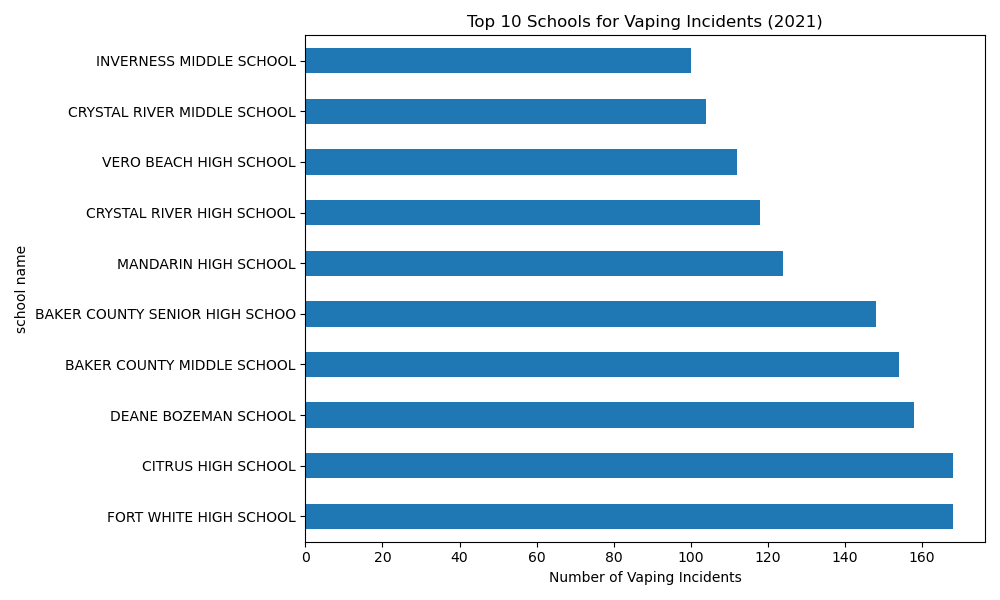
\includegraphics[width=\linewidth]{top_schools_vaping.png}
\captionof{figure}{Top 10 schools with the highest vaping incidents in 2021.}
\vspace{0.5cm}

This figure uses data from the Florida DOE SESIR dataset (2021). 
It highlights the ten schools with the most vaping-related incidents. 
The results show that a relatively small group of schools accounts for 
a large portion of reported vaping cases, suggesting that the problem 
is more concentrated in specific locations.

\section*{Visualization 2: Top 10 Districts for Vaping Incidents (2021)}
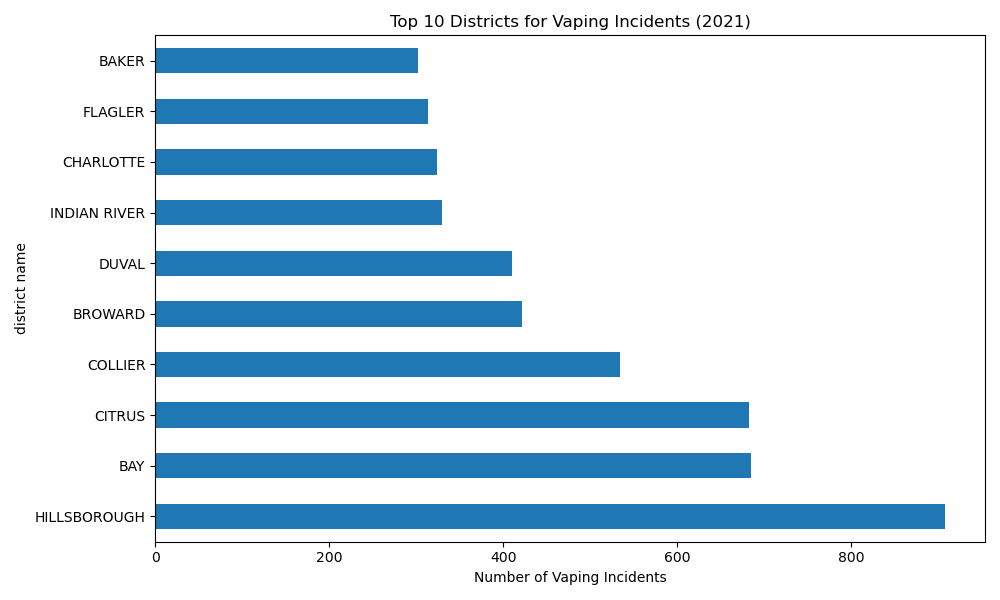
\includegraphics[width=\linewidth]{top_districts_vaping.png}
\captionof{figure}{Top 10 districts by vaping-related incidents in 2021.}
\vspace{0.5cm}

This figure also uses the Florida DOE SESIR dataset (2021), 
but aggregates incidents at the district level. 
It shows which districts have the highest reported totals of vaping-related cases. 
The visualization indicates that larger districts tend to report more cases, 
but some districts clearly stand out as hotspots compared to others.

\section*{Visualization 3: Vaping vs. Total Incidents (2021)}
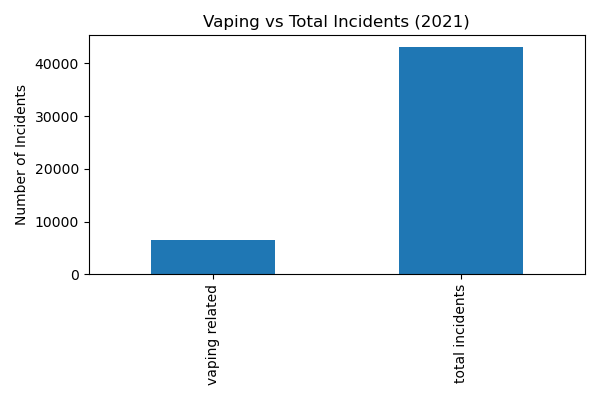
\includegraphics[width=0.7\linewidth]{vaping_vs_total.png}
\captionof{figure}{Comparison of vaping-related incidents to all reported incidents in 2021.}
\vspace{0.5cm}

This figure compares vaping incidents against the total number of all incidents 
in the 2021 dataset. While vaping is not the majority of school safety incidents, 
it represents a significant share of the overall problem. 
This emphasizes that vaping is one of the leading behavioral and safety concerns 
in Florida schools.

\end{document}
